\documentclass[../../main.tex]{subfiles}
\begin{document}
%
    In this chapter, we study the formation and breakage of bonds. We consider the simplest of models, where $N$ particles placed in a box interact through a pairwise potential.
    
    Potential functions come in many forms but usually provide two important features. First, they account for the resistance to compression, meaning that at a close range, we must have a repulsive force. Secondly, in order to bind particles together, it is necessary to include attraction over a certain range of separation.
    
\section{The Lennard-Jones Potential: Initial Look Into Bond Formation}

    The Lennard–Jones (L-J) potential, originally proposed for liquid argon \cite{jonesDeterminationMolecularFields1924}, provides a good starting point for our study. It is given by 
        \begin{equation}\label{eq: L-J - Lennard-Jones Potential}
            U_{\text{L-J}} = 4\epsilon \left[\left(\frac{\upsilon}{r}\right)^{12} - \left(\frac{\upsilon}{r}\right)^6\right] \,,
        \end{equation}
    where $r$ is the distance between particles, $\epsilon$ gives the depth of the well and so it is tied to the strength of the interaction, and $\upsilon$ gives the distance at which the potential is zero \cite{allenComputerSimulationLiquids2017}. Composed of just two terms, one dominating at short distances, modelling the repulsion between particles, and one attractive one, it became one of the most used potentials in MD for its computational simplicity.

    \begin{figure}[h]
        \centering
        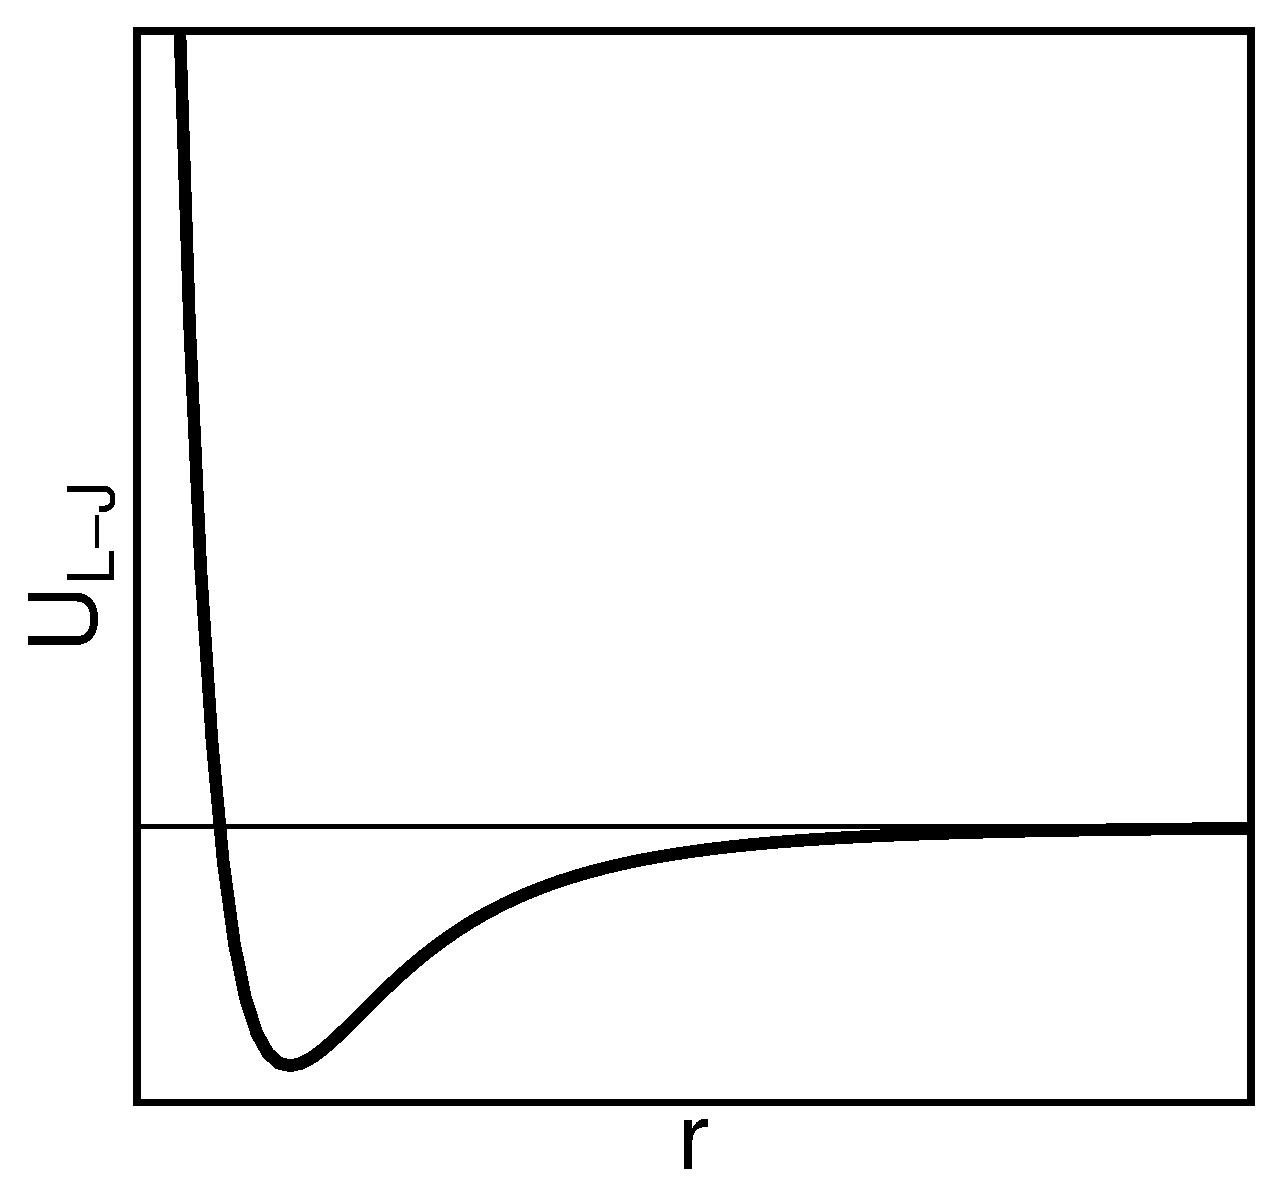
\includegraphics[scale = 0.4]{Figures/lj-pot.eps}
        \caption{Example of a typical Lennard-Jones potential.}
        \label{fig: L-J Potential}
    \end{figure}
    
    We set a cut-off radius that defines the distance at which the particles can interact (see \cref{app: Potential Cutt-off}). This ensures that the computational effort for one of the more demanding parts of our simulation, the calculation of the force, is reduced. When setting \textbf{P}eriodic \textbf{B}oundary \textbf{C}onditions (PBC) and \textbf{M}inimum \textbf{I}mage \textbf{C}onvention (MIC) we create replicas of our system in all directions and force the particles placed in the main box to interact with the closest particle images available (see \cref{app: PBC & MIC}). Failing to set a cut-off radius, or, for that matter, choosing a very small box, leads to numerical errors that arise from particles interacting with themselves since they are able to ``reach" their own images.
    
    We follow what is done in the vast majority of MD simulations that consider this potential \cite{allenComputerSimulationLiquids2017} and set the cut-off radius at
        \begin{equation}
            r_c = 2.5\,r_{min}\,, \ \text{where} \,\; r_{min} = 2^{1/6}\upsilon \,. 
        \end{equation} 
    
    The motion of each of these particles will be given by
        \begin{equation}
            \zeta \frac{d\mathbf{R}_n}{dt} = \bm{\xi}_n + \sum_{m \neq n} \mathbf{f}_{nm}\,,
        \end{equation}
    where $\mathbf{f}_{nm}$ is the force exerted upon particle $n$ by particle $m$,
        \begin{equation}\label{eq: L-J - Chain Rule-Force}
        \begin{split}
            \mathbf{f}_{nm} &= - \frac{\partial U_{\text{L-J}}}{\partial \mathbf{r}_{nm}} = -\frac{\mathbf{r}_{nm}}{r_{nm}}\frac{\partial U_{\text{L-J}}}{\partial r_{nm}} = \\
            &= \left(\frac{\mathbf{r}_{nm}}{r_{nm}^2}\right)\,\left\{ 48\epsilon \left[ \left(\frac{\upsilon}{r_{nm}}\right)^{12} - \frac{1}{2}\left(\frac{\upsilon}{r_{nm}}\right)^6 \right]\right\} \,,
        \end{split}
        \end{equation}
    with $\mathbf{r}_{nm} = \mathbf{R}_n - \mathbf{R}_m$ as the distance between the two particles.
\begin{comment}
    The motion of each of these particles will be given by
        \begin{equation}
            \zeta \frac{d\mathbf{R}_n}{dt} = \bm{\xi}_n - \sum_{\substack{m=1\\ m \neq n}}^{N} \bm{\nabla}_{nm}\,U_{\text{L-J}} \,.
        \end{equation}
    By making use of the chain rule we have that
        \begin{equation}\label{eq: L-J - Chain Rule-Force}
        \begin{split}
            \bm{\nabla}_{nm}\,U_{\text{L-J}} &= - \frac{\partial U_{\text{L-J}}}{\partial \mathbf{r}_{nm}} = -\frac{\mathbf{r}_{nm}}{r_{nm}}\frac{\partial U_{\text{L-J}}}{\partial r_{nm}} = \\
            &= \left(\frac{\mathbf{r}_{nm}}{r_{nm}^2}\right)\,\left\{ 48\epsilon \left[ \left(\frac{\upsilon}{r_{nm}}\right)^{12} - \frac{1}{2}\left(\frac{\upsilon}{r_{nm}}\right)^6 \right]\right\} \,,
        \end{split}
        \end{equation}
    where $\mathbf{r}_{nm} = \mathbf{R}_m - \mathbf{R}_n$ is the distance between the two particles. 
\end{comment}        

    We first study the effect of temperature on the type of clusters formed, by measuring the number of bonds per particle, $\Upsilon$, the rate, $k$, at which those are formed, or broken, and, in a more qualitative manner, the type of structures that are formed.
    
    In order to achieve this, it is imperative that we first define what is a bond. For this simple potential, two particles are bonded if the distance between the two is less than the cut-off radius $r_c$.
\begin{comment}
            %
        \begin{figure}[h]
            \centering
            \begin{subfigure}[b]{0.475\textwidth}
                \centering
                \includegraphics[width=\textwidth]{Figures/begin_np.png}
                \caption{Corresponds to the start of the simulation. The particles have just been randomly set inside the box, taking measures to avoid overlapping.}
                \label{fig: initial condition}
            \end{subfigure}
            \hfill
            \begin{subfigure}[b]{0.475\textwidth}
                \centering
                \includegraphics[width=\textwidth]{Figures/end_np.png}
                \caption{Corresponds to the end of the simulation. An equilibrium in the number of bonds per particle has been reached.}
                \label{fig: end of simul vmd}
            \end{subfigure}
            \caption{The two images here shown were grabbed from a video of the many systems studied during this work. The particles correspond to the orange ``dots" while the blue ``lines" show a formed bond. During the video, as the bonds are formed and broken, the lines will appear and disappear proving an invaluable tool in error detection and correction, as well as in the understanding of the system.}
            \label{fig: vmd screen}
        \end{figure}
\end{comment}
    %
        \begin{figure}[h]
            \centering
            \begin{subfigure}[b]{0.475\textwidth}
                \centering
                \includegraphics[width=\textwidth]{Figures/begin_np.png}
                \caption{}
                \label{fig: initial condition}
            \end{subfigure}
            \hfill
            \begin{subfigure}[b]{0.475\textwidth}
                \centering
                \includegraphics[width=\textwidth]{Figures/end_np.png}
                \caption{}
                \label{fig: end of simul vmd}
            \end{subfigure}
            \caption{The two images are snapshots of one of the systems studied. The orange ``dots" correspond to the particles and the blue ``lines" represent the bonds formed by those particles at the time the snapshot was taken. The start of the simulation is shown in \cref{fig: initial condition}. The particles are randomly set inside the box, taking measures to avoid overlapping. In \cref{fig: end of simul vmd} we show the end of the simulation where an equilibrium in the number of bonds per particle has been reached. Having a visual representation of the system proved to be an invaluable tool in error detection and correction, as well as in the understanding of the system.}
            \label{fig: vmd screen}
        \end{figure}
        
    The position of each particle is set at random inside the simulation box, with special care to avoid overlapping. This can be noted in \cref{fig: vmd screen}, where it is shown the initial state as well as the final one, where an equilibrium has been reached. We define this as the time where $\Upsilon$ stays stable. 
        
    It was to be expected that an increase in temperature would result in fewer bonds since a decrease in thermal fluctuations will, in theory, trap the particles in the potential well. In \cref{fig: L-J temperature in number of bonds} we show that for a low temperature (\cref{fig: LJ - half g}), a particle will form on average around eleven bonds. Such a high number of bonds was not expected considering that, at short ranges, the particles should repel each other, preventing such highly connected clusters. We notice that by setting the distance as far as $r_c$ led us to count a sort of ``next nearest neighbours" as a bond. This is not realistic and is a consequence of a greater problem: the potential chosen.    
\begin{comment}
    What was not expected was the large value for $\Upsilon_{eq}$ at low temperatures. Setting the distance as far as $r_c$ has led to us to count a sort of ``next nearest neighbours" as a bond. This isn't incorrect in itself. It is a direct consequence of a greater problem: the potential chosen.    
\end{comment}    
    %
        \begin{figure}[h]
            \centering
            \begin{subfigure}[b]{0.328\textwidth}
                \centering
                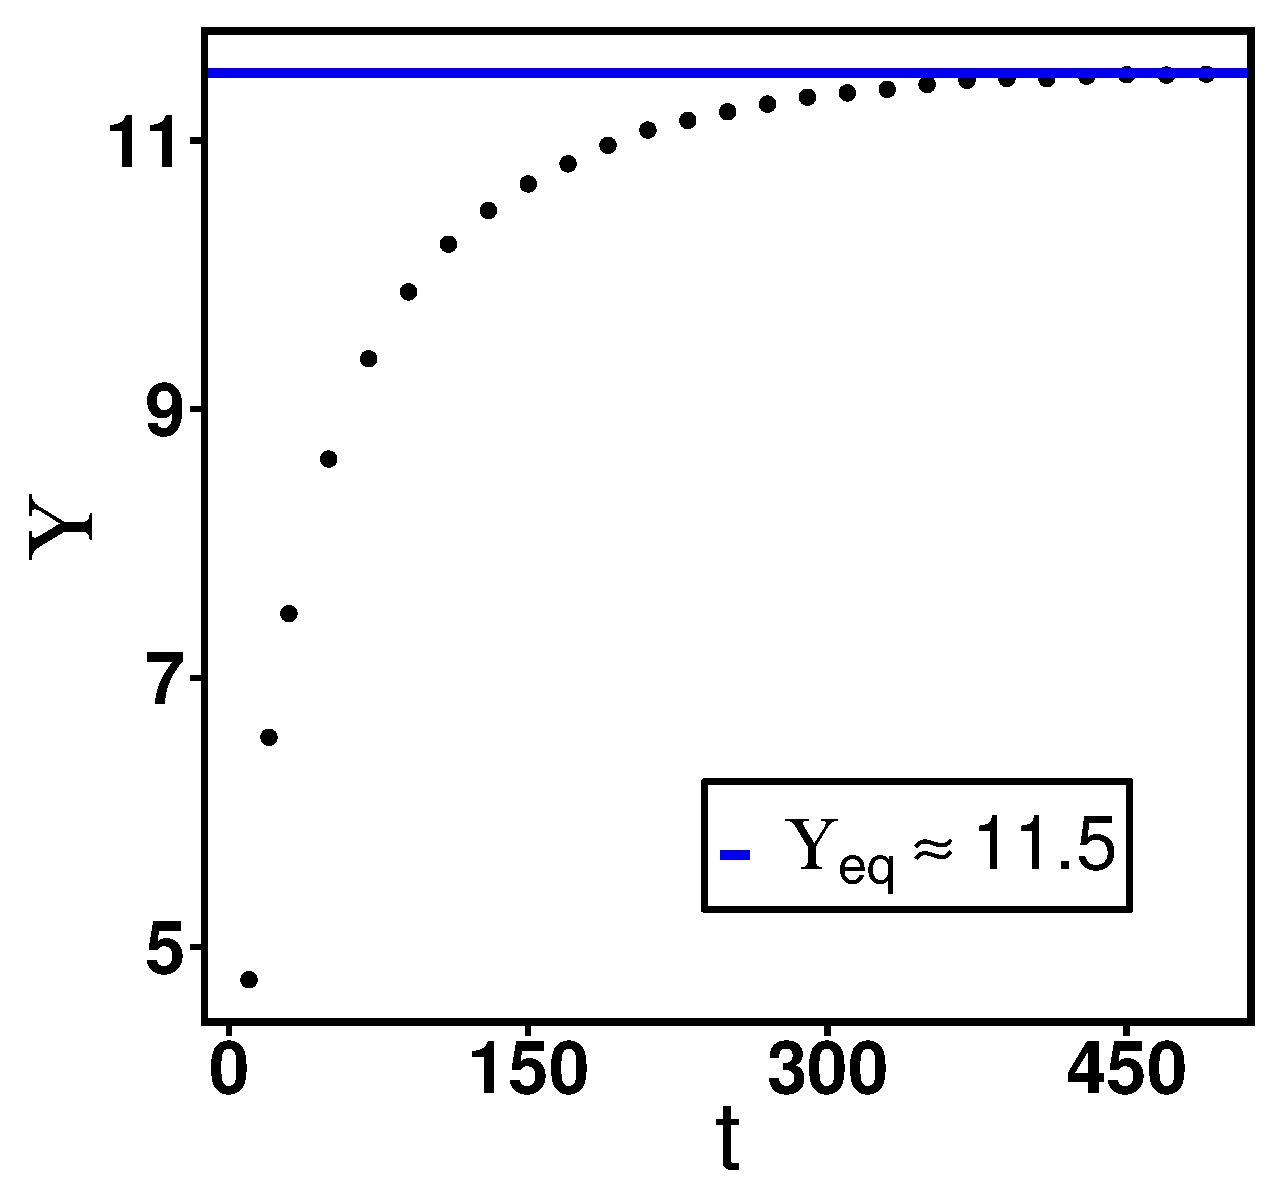
\includegraphics[width=\textwidth]{Figures/lj_halfg.eps}
                \caption{$g = 0.5$}
                \label{fig: LJ - half g}
            \end{subfigure}
            \hfill
            \begin{subfigure}[b]{0.328\textwidth}
                \centering
                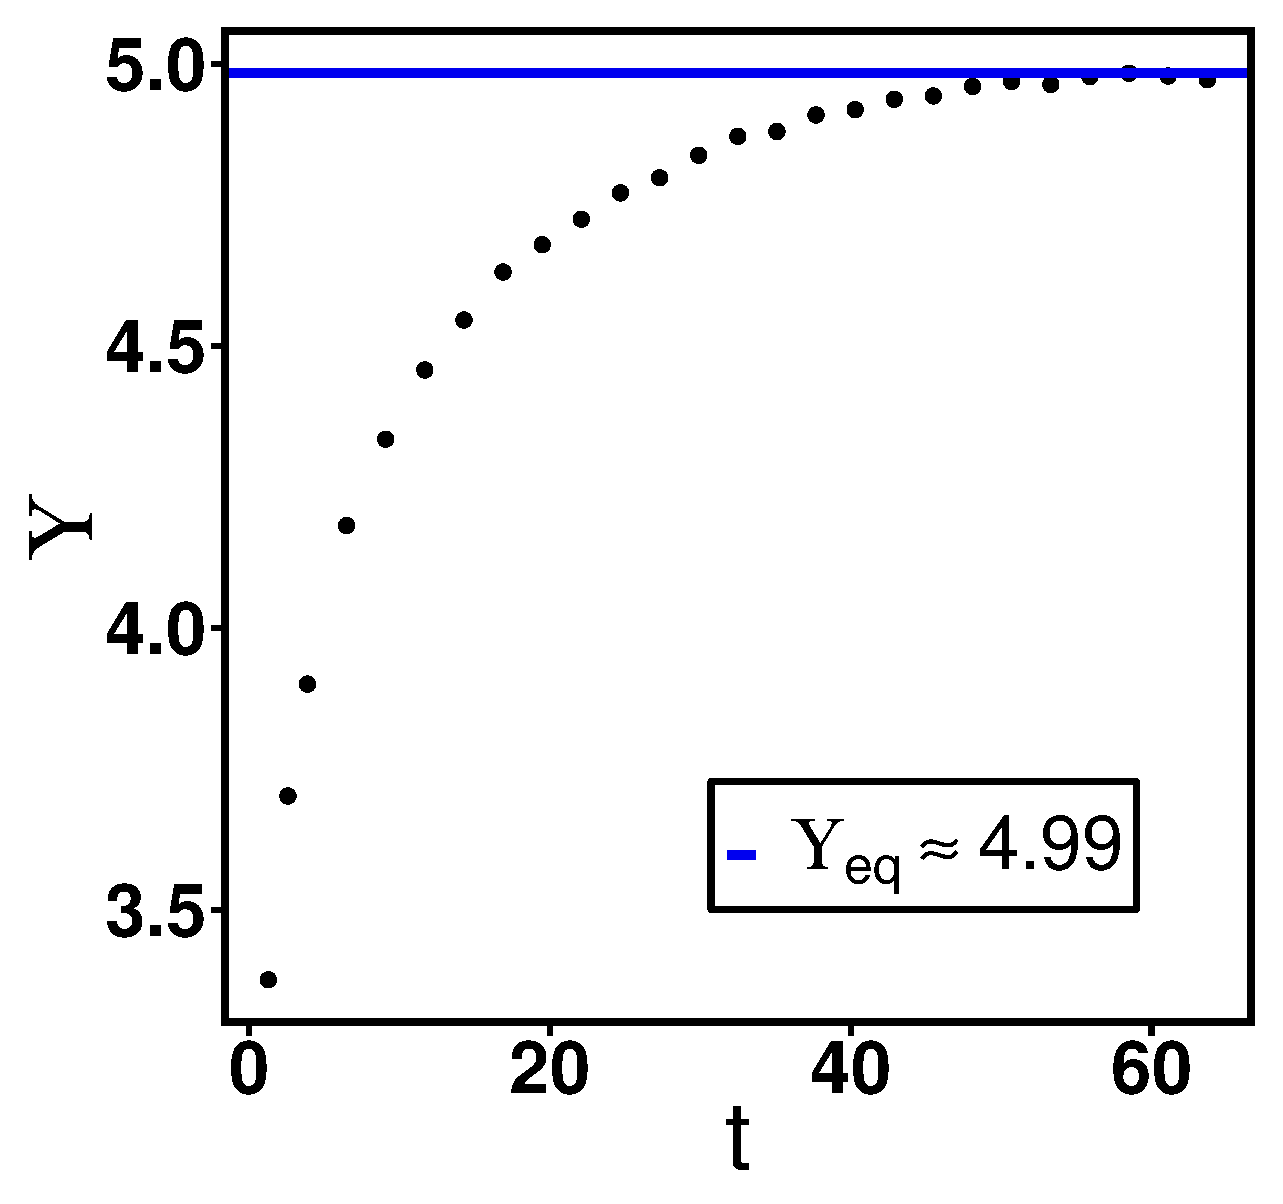
\includegraphics[width=\textwidth]{Figures/lj_oneg.eps}
                \caption{$g = 1$}
                \label{fig: LJ - one g}
            \end{subfigure}
            \begin{subfigure}[b]{0.328\textwidth}
                \centering
                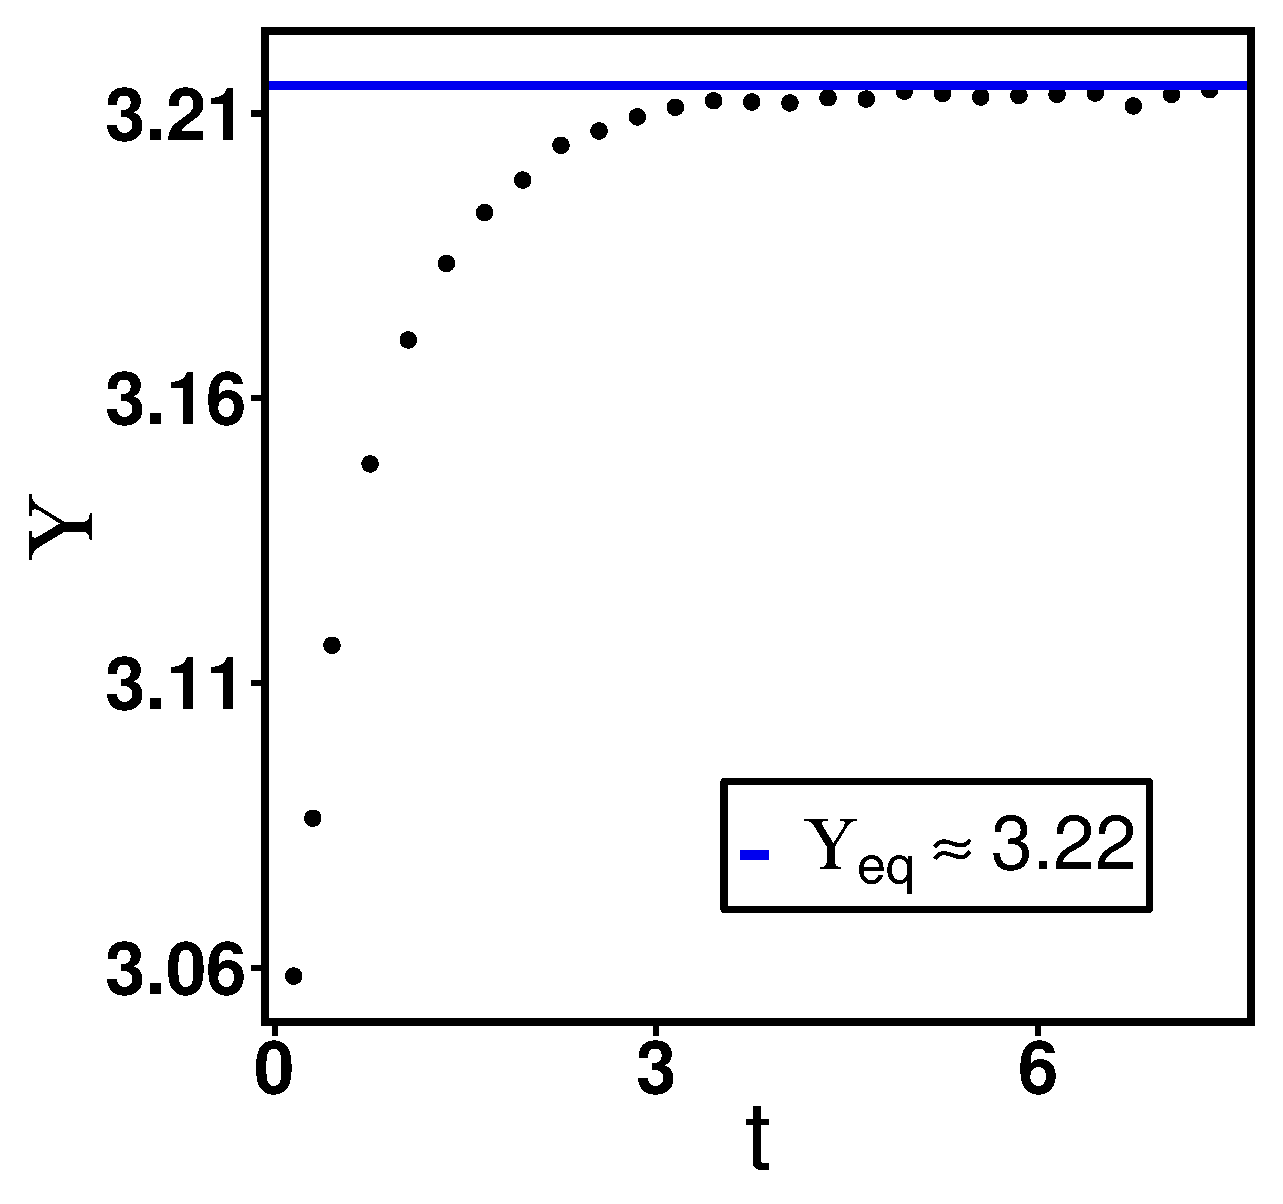
\includegraphics[width=\textwidth]{Figures/lj_twog.eps}
                \caption{$g = 2$}
                \label{fig: LJ - two g}
            \end{subfigure}
            \caption{Comparison between 3 simulations using the L-J potential. We see that as the temperature increases, the number of bonds each particle makes and the time the system takes to reach an equilibrium position, \textit{i.e.} the relaxation time, decrease. We can also observe a very high $\Upsilon_{eq}$ for the case of \cref{fig: LJ - half g}. Parameters used: $\upsilon = 1$, $\epsilon = 1$, $\rho = 2/15$ [\cref{eq: Lennard-Jones - density}].}
            \label{fig: L-J temperature in number of bonds}
        \end{figure}
        


\section{A New Potential: Influence of Temperature and Density on Bond Formation}
\begin{comment}
    The L-J potential lacks a activation barrier for the formation of a bond making it possible for one particle to ``dance" around the cut-off region, on what amounts to flipping the on and off switch of that particular bond since, at this distance, the resulting forces acting upon the particle are negligible. By introducing an energy barrier with a clear cost to form a bond this is avoided. We can now too, if we so choose, set the formation of a bond at a much shorter distance with a clear physical meaning behind it.
\end{comment}
    The L-J potential lacks a activation barrier for the formation of a bond. This is unrealistic and poses a challenge to the definition of a bond. 
    
    We address this by adding an exponential to the L-J potential [\cref{eq: L-J - Lennard-Jones Potential}], including a clear cost for the formation of a bond in the form of an energy barrier. We thus define the potential, $U_\beta$, as
        \begin{equation}\label{eq: L-J - New Potential}
            U_{\beta} = 4\epsilon \left[\left(\frac{\upsilon}{r}\right)^{12} - \left(\frac{\upsilon}{r}\right)^6\right] + h\exp \left[ -\frac{\left(r - r_b\right)^2}{w^2} \right]\,,
        \end{equation}
    where $h$ and $w$ are the height and width of the potential wall, respectively, and $r_b$ is the point where we define the formation/breakage of the bond, corresponding to the local maximum of the function (\cref{fig: newpot}).
    
    The force will be calculated through the same steps previously described in \cref{eq: L-J - Chain Rule-Force} to get
        \begin{equation}
            \bm{\nabla}_n\,U_{\beta} = \left( \frac{\mathbf{r}_n}{r_n^2} \right)\,\left\{ 48\epsilon \left[\left( \frac{\upsilon}{r_n} \right)^{12} - \frac{1}{2} \left( \frac{\upsilon}{r_n} \right)^6 \right] +  \frac{2h \left( r_n - r_b \right)}{w^2}\exp\left[ -\frac{(r_n - r_b)^2}{w^2} \right] \right\} \,.
        \end{equation}
        \begin{figure}[h]
            \centering
            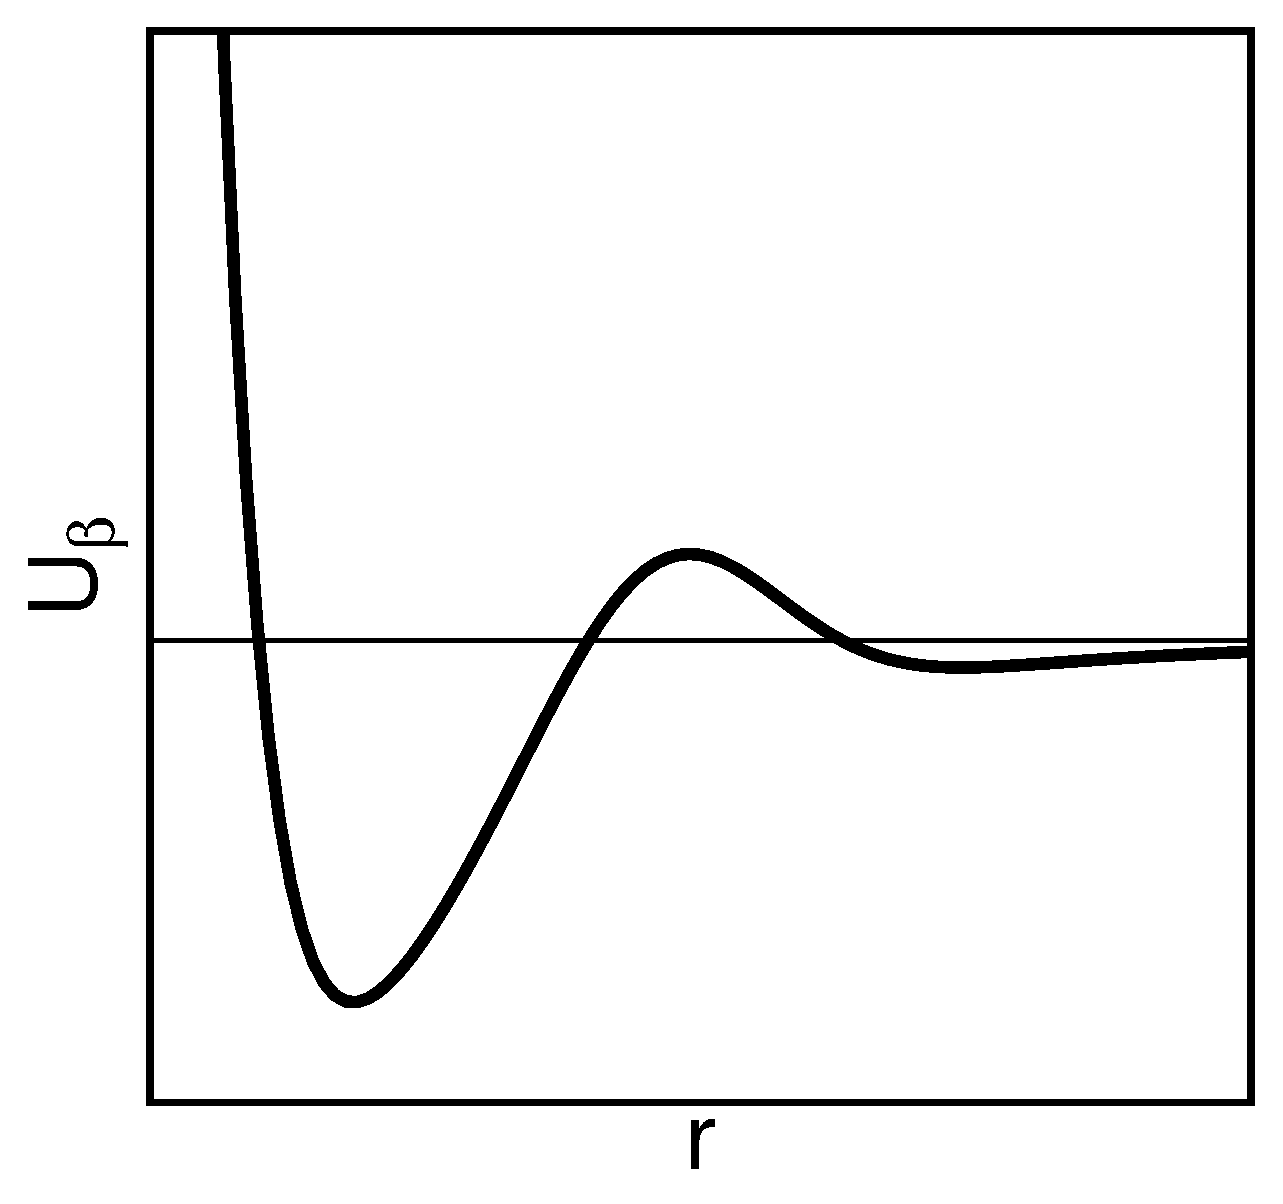
\includegraphics[scale = 0.4]{Figures/newpot.eps}
            \caption{Example of the new potential based on the L-J with an additional Gaussian curve}
            \label{fig: newpot}
        \end{figure}
        
    We start with a simple test on the particle-particle interactions. In one dimension, we fix a particle, allowing another to move, interacting with the previous one through the potential. We can time how long it takes for it to go from the starting distance, which we set as $r_{min}$, to $r_b$, meaning, the time it takes for a formed bond to break.
    
    In chemical kinetics, the Arrhenius equation is used to compute the temperature dependence of the reaction rate
    \begin{equation}
        k = A \exp\left(\frac{E_a}{k_bT}\right) \,,
    \end{equation}
    where $k$ is the rate constant, $A$ is some pre-exponential factor and $E_a$ is the activation energy, which is the minimum energy necessary in order to form a bond.
    
    For a single rated-limited activated process, the plot of the logarithm of a reaction rate against the inverse of the temperature will give a straight line whose slope can be used to find $E_a$.
        \begin{equation}\label{eq: Lennard-Jones - Arrhenius plot equation (I)}
            \log(k) = \log(A) + \frac{E_a}{k_B}\frac{1}{T} \,.
        \end{equation}
    
    If we define our rate constant $k$ as the average time needed for our particle to escape the potential well, by varying $g$, the activation energy for a bond to break, $E_{a,b}$, should correspond to the difference in energy between our starting point, $r_{min}$, and the point where the particle breaks its bond, $r_b$. Substituting $g$ into \cref{eq: Lennard-Jones - Arrhenius plot equation (I)} we obtain
        \begin{equation}\label{eq: Lennard-Jones - Arrhenius plot equation (II)}
            \log(k) = \log(A) + 2\zeta E_{a,b}\frac{1}{g} \,.
        \end{equation}
        
    The value of the potential will depend on the parameters used and on where we define the distance at which we set the barrier. In order to facilitate a comparison to \cref{fig: arrhenius}, the same parameters are used. The expected activation energy, $E_{a, b}^t$, will be
        \begin{equation}\label{eq: Lennard-Jones - Arrhenius plot equation (value)}
            E_{a,b}^t = U_{\beta}(r_b) - U_{\beta}(r_{min}) = 1.445 \,,
        \end{equation}
    in units of $\epsilon$.
    
    From \cref{fig: arrhenius}, we know that the value of the slope is close to $E_{a,b}^t$. The small deviation from the expected value is due to the fact that, for some samples, the simulation time was not long enough for the bond to break
        \begin{figure}[h]
            \centering
            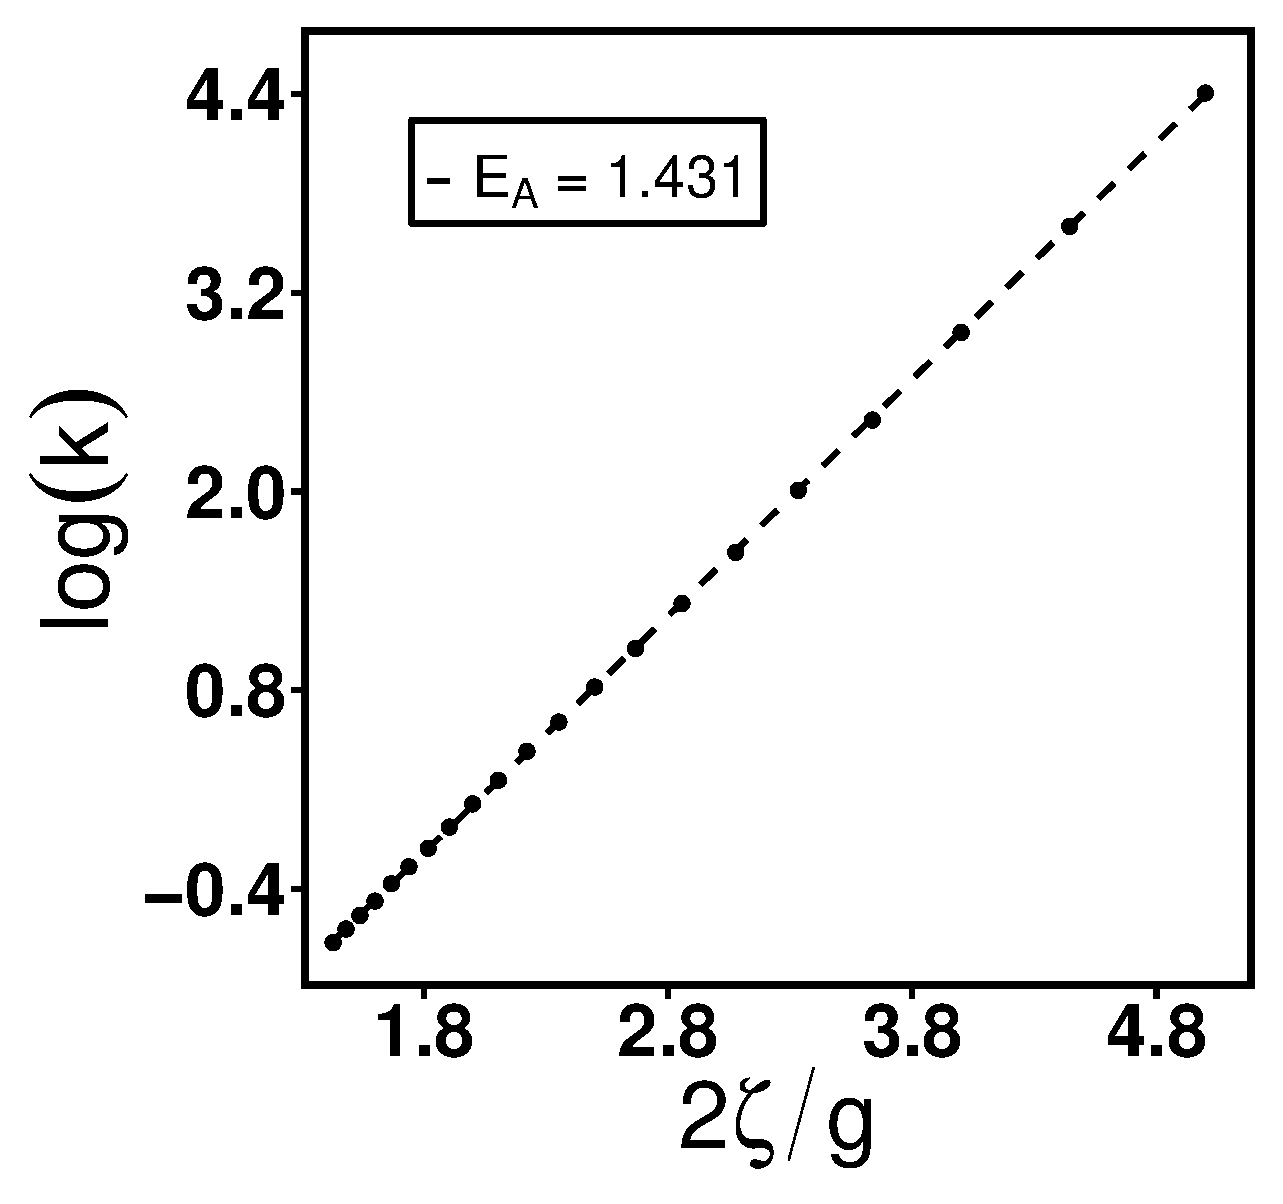
\includegraphics[scale = 0.4]{Figures/Arrhenius.eps}
            \caption{In 1D, we time how long a particle takes to reach $r_b$ after it was initially set at $r_{min}$. After this has been sampled numerous times and the results averaged out, the temperature is increased and the process repeated. By plotting the logarithm of the rate at which the bonds are broken against the temperature change, the resulting slope should give the potential difference between the two points (\cref{eq: Lennard-Jones - Arrhenius plot equation (II),eq: Lennard-Jones - Arrhenius plot equation (value)}). Parameters used: $\upsilon = 1$, $\epsilon = 1$, $h = 0.8$, $w = 0.15$, $r_b = 1.52$.}
            \label{fig: arrhenius}
        \end{figure}
    
    By shortening the distance at which we define the particles as bonded, we can immediately expect that the number of bonds formed will fall when compared to the previous case shown in \cref{fig: L-J temperature in number of bonds}. It is however interesting to note that it appears to exist a sort of optimal $g$ for which $\Upsilon_{eq}$ is maximum and that, past a certain point, the increase in $g$ does not seem to lead to a significant change in $\Upsilon_{eq}$. As a result of the small number of cases studied, the exploratory study made with the L-J potential [\cref{eq: L-J - Lennard-Jones Potential}] failed to show this behaviour.
    %
        \begin{figure}[h]
            \centering
            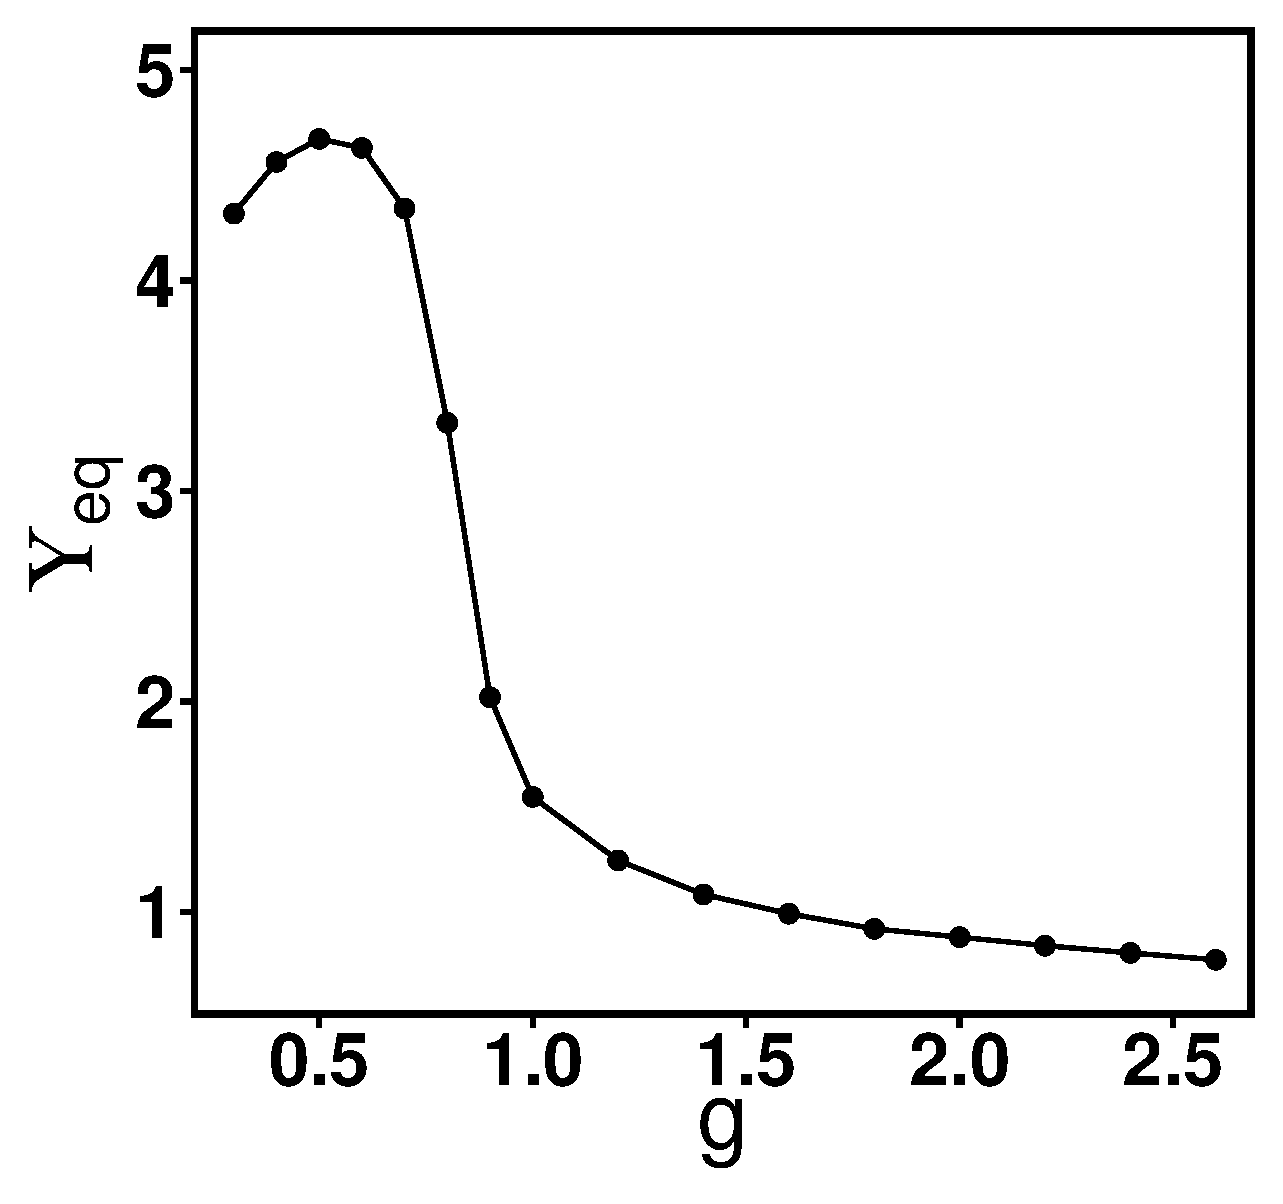
\includegraphics[scale=0.4]{Figures/np_g.eps}
            \caption{We show here the effect temperature has on the number of bonds formed. In its initial state, all particles are placed at random with the only condition being no overlapping. We then let the system relax until a state where the number of bonds formed is kept more or less the same, $\Upsilon_{eq}$. We show that, for the parameters used, there is a optimal $g$ at which $\Upsilon_{eq}$ is maximum. This is most likely explained by the rate for the formation and breakage of bonds, which is in turn a result of the type of potential used. Parameters used: $\upsilon = 1$, $\epsilon = 1$, $h = 0.8$, $w = 0.15$, $r_b = 1.52$, $\rho = 2/15$.}
            \label{fig: np2D - n bonds (g)}
        \end{figure}
    
    We explain this phenomenon by a simple rule: the increase/decrease in the magnitude of thermal fluctuations results in an increase/decrease in the probability of a particle crossing the potential barrier laid out before it. There are two different limiting behaviours: for a low $g$, thermal fluctuations are small enough to trap the system in its initial configuration, meaning that the rate at which bonds are formed/destroyed is much smaller; for a high $g$, thermal fluctuations become large enough to make the potential well/barrier negligible, so particles will form and break bonds without a clear cost for it, since the random thermal forces will dominate over their interactions with the other particles in the medium. The fact that we observe a maximum at $g \approx 0.5$ is due to the difference in cost between forming a bond (low cost) and breaking it (high cost) [\cref{eq: L-J - New Potential}].  
    %
        \begin{figure}[h]
            \centering
            \begin{subfigure}[b]{0.45\textwidth}
                \centering
                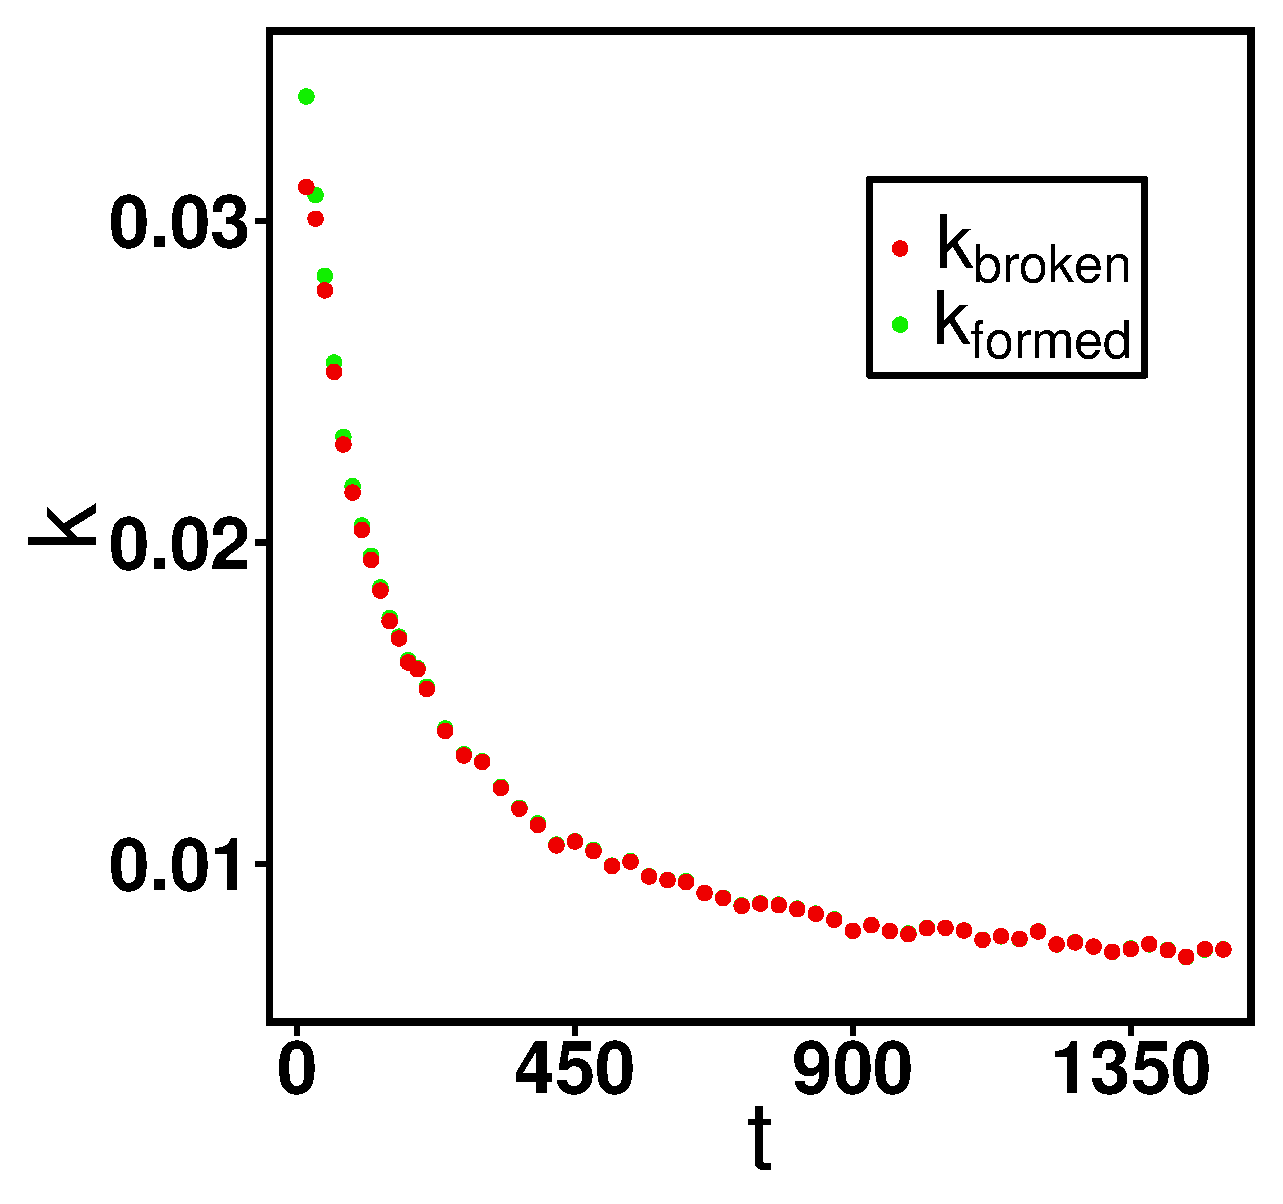
\includegraphics[width=\textwidth]{Figures/rate_g060.eps}
                \caption{$g=0.60$}
                \label{fig: np2D - rate (g=0.60)}
            \end{subfigure}
            \hfill
            \begin{subfigure}[b]{0.45\textwidth}
                \centering
                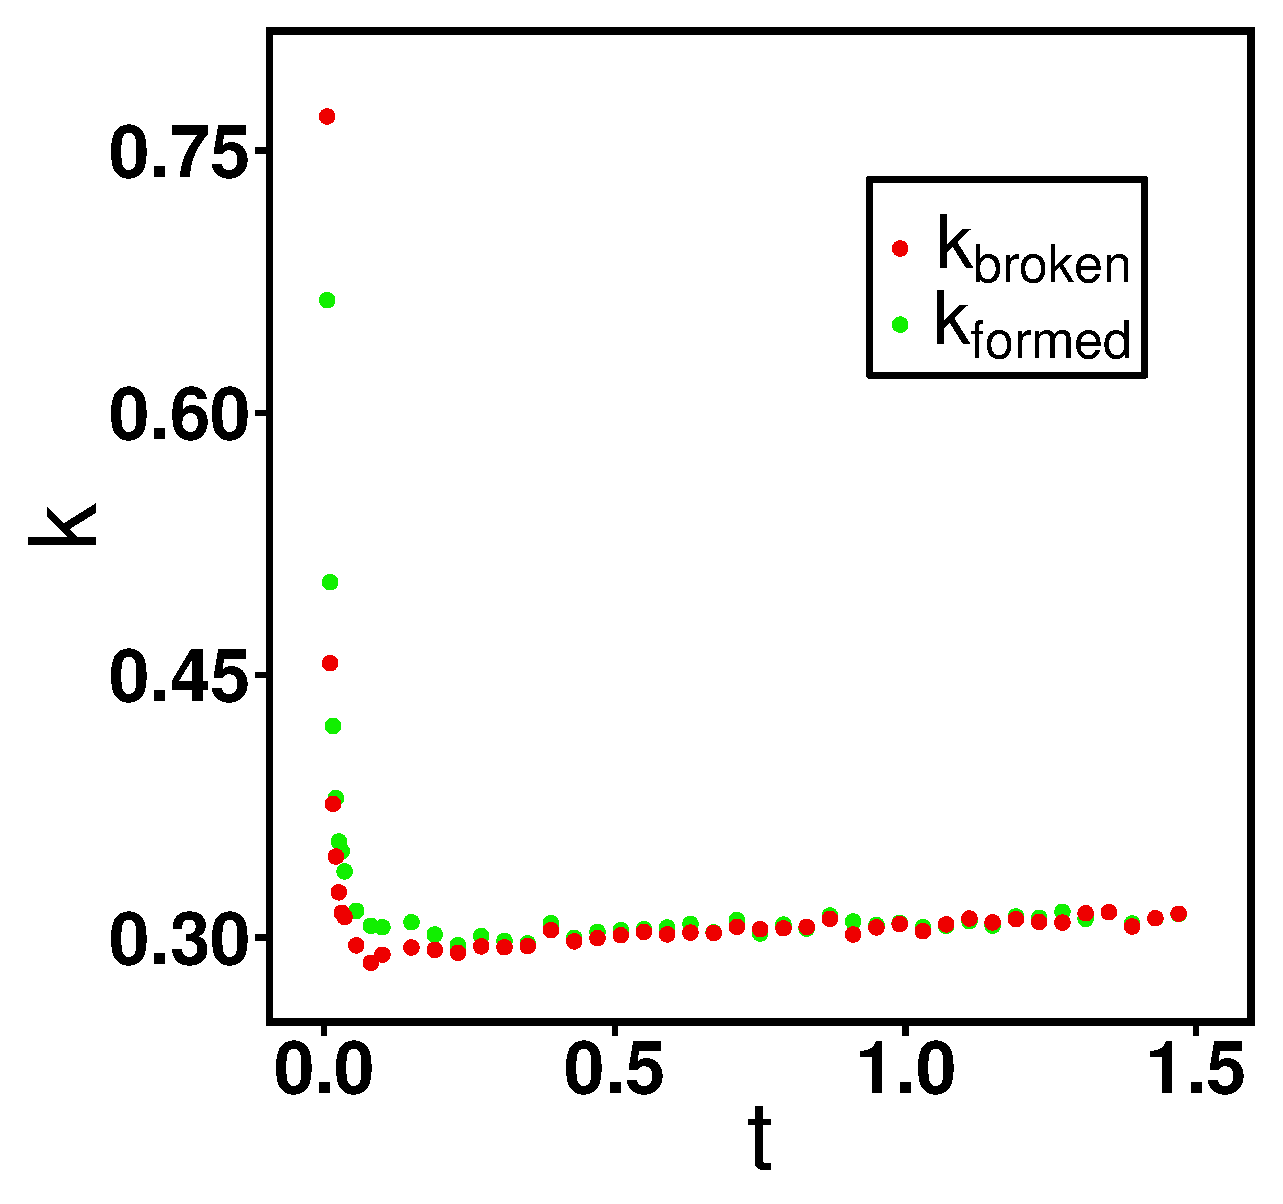
\includegraphics[width=\textwidth]{Figures/rate_g150.eps}
                \caption{$g = 1.50$}
                \label{fig: np2D - rate (g=1.50)}
            \end{subfigure}
            \caption{The effect of temperature on the rates for bond formation and breakage. We show that for $g = 0.60$ it takes much longer to reach the equilibrium state where $k_{formed}$ and $k_{broken}$ are equal. We observe that, before this occurs, $k_{formed} > k_{broken}$, showing that from our initial state, we would see a rise in $\Upsilon$ . We also note that the rate of either events is lower in the case of $g=0.6$, by a factor of $10$. This was to be expected since the energy cost for both events is kept the same for both cases ($E_{a, b} = 1.445$ and $E_{a, f} = 0.502$). What is shown can serve as an addendum to \cref{fig: np2D - n bonds (g)}, giving valuable insight to better understand the results there shown. Parameters used: $\upsilon = 1$, $\epsilon = 1$, $h = 0.8$, $w = 0.15$, $r_b = 1.52$, $\rho = 2/15$.}
            \label{fig: np2D - rate}
        \end{figure}     

    In \cref{fig: np2D - rate}, we compare the rate, $k$, at which bonds are formed and broken for different $g$. We observe that the rates $k_{formed}$ and $k_{broken}$ are indeed much smaller for a low $g$ in an equilibrium regime, solidifying our previous conclusion. Another thing to note is the time scale in which this process occurs, showing that for low $g$, the system takes much longer to reach an equilibrium state between the two rates ($k_{formed}$ and $k_{broken}$), leading to a greater number of bonds formed (\cref{fig: np2D - n bonds (g)}). 
    
    Let us now focus on the effect of the density, defined as
        \begin{equation}\label{eq: Lennard-Jones - density}
            \rho = \frac{N}{A} \,,
        \end{equation}
    where $A$ is the area of our enclosing box and $N$ is the number of particles. Driving the choice of density used were the rules we set for the initial state of the system and the amount of events that were observed. Regarding the first case, we set a maximum to how closely we could pack the particles since otherwise, the time to generate the initial configuration would diverge when approaching the jammed state. The second case refers to the fact that at low $\rho$ the number of bonds formed is very low, with the particles wandering in the free space available meaning the system will take much longer to form bonds and converge to a stationary state.
    %
        \begin{figure}[h]
            \centering
            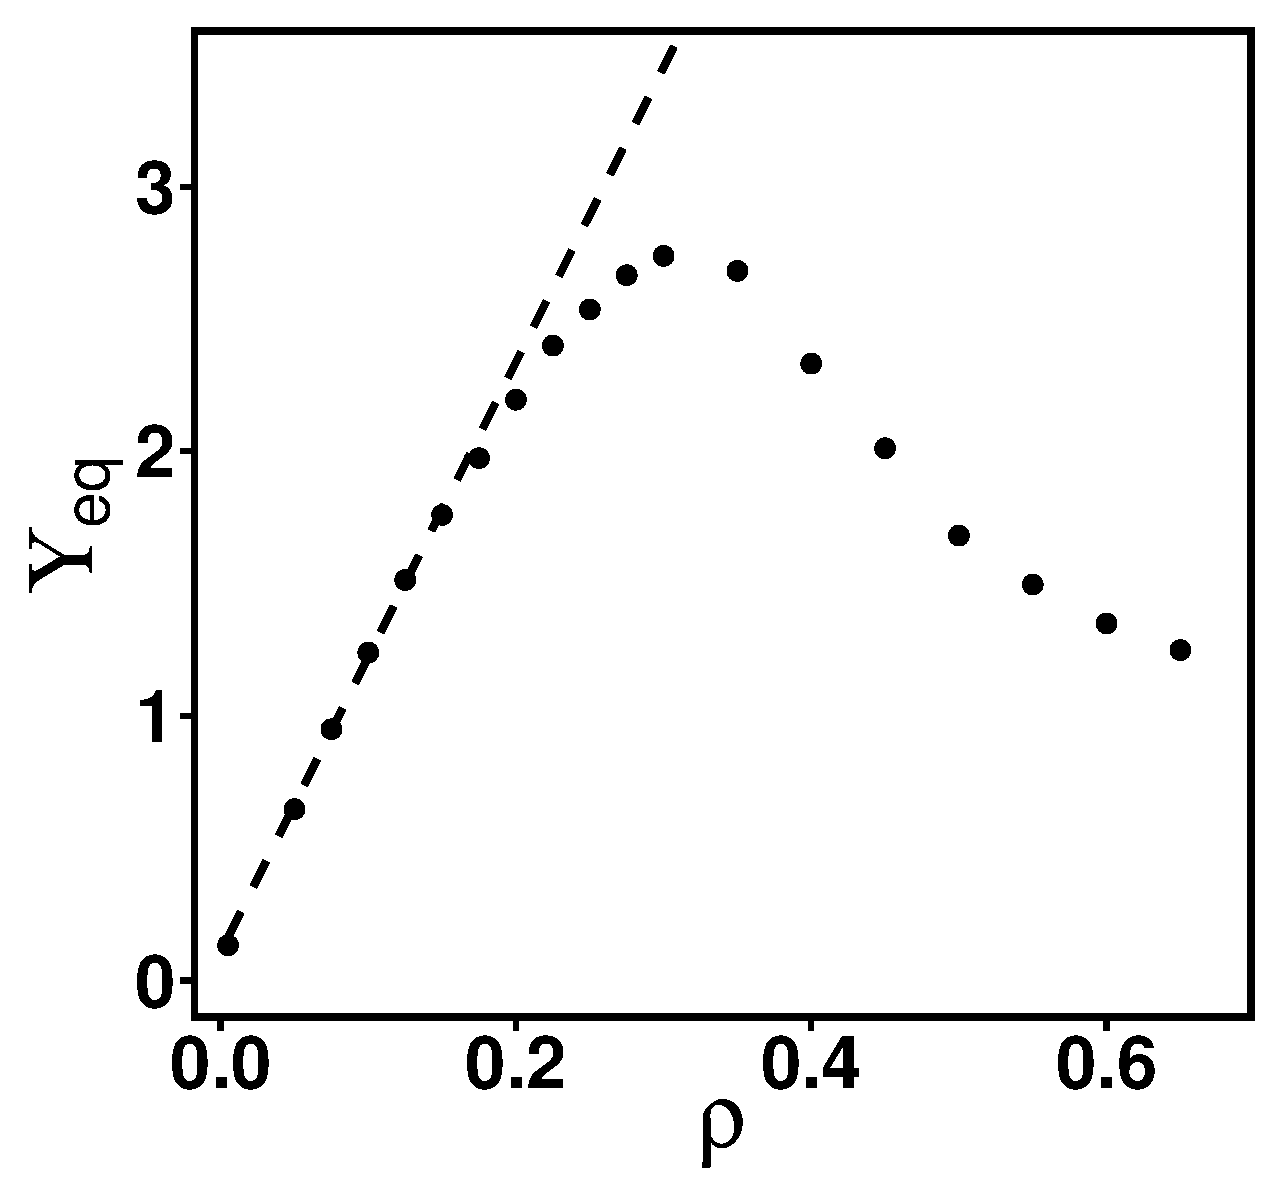
\includegraphics[scale=0.4]{Figures/np2D_rho.eps}
            \caption{The effect of particle density, $\rho$, on the number of bonds formed. We use a high density of particles throughout this work in order to reduce the amount of computational time it takes for a system to reach its relaxed state. Note the linear relation between the two quantities for low $\rho$ used in the rest of this work. Parameters used: $g = 1$, $\upsilon = 1$, $\epsilon = 1$, $h = 0.8$, $w = 0.15$, $r_b = 1.52$.}
            \label{fig: np2D - rho}
        \end{figure}
    
    In \cref{fig: np2D - rho} we show the relation between $\Upsilon_{eq}$ and $\rho$. Two distinct regimes are observed with a soft transition between the two. We note that, for small $\rho$, $\Upsilon_{eq}$ increases linearly. As the space where particles can diffuse freely gets tighter, they are ``forced" to come together and form bonds. For $\rho \gtrsim 0.35$, the decay in $\Upsilon_{eq}$ may be explained by a diminishing kinetic energy caused by a balancing act between the thermal motion and the energy cost of closing in on multiple particles. In other words, their motion is set to a minimum due to interactions with neighbouring particles.
    
    We have discussed the necessity of adding a cost to the formation of a bond. We now observe that it has led to a smaller $\Upsilon_{eq}$, as predicted; that, in spite of an initial assumption on the role played by temperature and density, there is not a direct relation to the size of aggregates formed and that this behaviour is in part explained by the potential barrier added. It is important to note that by keeping a low density of particles, the computational time can be reduced considerably. 
%
\end{document}